



\documentclass[
	% -- opções da classe memoir --
	12pt,				% tamanho da fonte
	openright,			% capítulos começam em pág ímpar (insere página vazia caso preciso)
	oneside,			% para impressão em recto e verso. Oposto a oneside
	a4paper,			% tamanho do papel. 
	% -- opções da classe abntex2 --
	%chapter=TITLE,		% títulos de capítulos convertidos em letras maiúsculas
	%section=TITLE,		% títulos de seções convertidos em letras maiúsculas
	%subsection=TITLE,	% títulos de subseções convertidos em letras maiúsculas
	%subsubsection=TITLE,% títulos de subsubseções convertidos em letras maiúsculas
	% -- opções do pacote babel --
	english,			% idioma adicional para hifenização
	french,				% idioma adicional para hifenização
	spanish,			% idioma adicional para hifenização
	brazil				% o último idioma é o principal do documento
	]{abntex2}




% Pacotes básicos 
\usepackage{lmodern}			% Usa a fonte Latin Modern			
\usepackage[T1]{fontenc}		% Selecao de codigos de fonte.
\usepackage[utf8]{inputenc}		% Codificacao do documento (conversão automática dos acentos)
\usepackage{indentfirst}		% Indenta o primeiro parágrafo de cada seção.
\usepackage{color}				% Controle das cores
\usepackage{graphicx}			% Inclusão de gráficos
\usepackage{microtype} 			% para melhorias de justificação
\usepackage{amsmath}			% lib para equacoes
\usepackage{svg}
\usepackage{listings}
\usepackage{verbatim}
%\usepackage{float}


% Pacotes adicionais, usados apenas no âmbito do Modelo Canônico do abnteX2

\usepackage{lipsum}				% para geração de dummy text



% Pacotes de citações
\usepackage[num, backend=biblatex]{abntex2cite}	% Citações padrão ABNT
\usepackage[brazilian,hyperpageref]{backref}	 % Paginas com as citações na bibl


\definecolor{mGreen}{rgb}{0,0.6,0}
\definecolor{mGray}{rgb}{0.5,0.5,0.5}
\definecolor{mPurple}{rgb}{0.58,0,0.82}
\definecolor{backgroundColour}{rgb}{0.95,0.95,0.92}

 
% CONFIGURAÇÕES DE PACOTES

% Configurações do pacote listings
\lstdefinestyle{CStyle}{
    backgroundcolor=\color{backgroundColour},   
    commentstyle=\color{mGreen},
    keywordstyle=\color{magenta},
    numberstyle=\tiny\color{mGray},
    stringstyle=\color{mPurple},
    basicstyle=\footnotesize,
    breakatwhitespace=false,         
    breaklines=true,                 
    captionpos=b,                    
    keepspaces=true,                 
    numbers=left,                    
    numbersep=5pt,                  
    showspaces=false,                
    showstringspaces=false,
    showtabs=false,                  
    tabsize=2,
    language=C
}

% Configurações do pacote backref
% Usado sem a opção hyperpageref de backref
\renewcommand{\backrefpagesname}{Citado na(s) página(s):~}
% Texto padrão antes do número das páginas
\renewcommand{\backref}{}
% Define os textos da citação
\renewcommand*{\backrefalt}[4]{
	\ifcase #1 %
		Nenhuma citação no texto.%
	\or
		Citado na página #2.%
	\else
		Citado #1 vezes nas páginas #2.%
	\fi}%
% ---



% ---
% Informações de dados para CAPA e FOLHA DE ROSTO
% ---
\titulo{Robô omnidirecional de 3 rodas}
\autor{Elton Mauricio da Silva}
\local{Brasil}
\data{2022}
\orientador{Marcelo Bender Perotoni}
\instituicao{%
  Universidade Federal do ABC
  \par
  CMCC
  \par
   Bacharelado em Ciência da Computação
}
\tipotrabalho{Tese (Doutorado)}
% O preambulo deve conter o tipo do trabalho, o objetivo, 
% o nome da instituição e a área de concentração 
\preambulo{ }



% Configurações de aparência do PDF final

% alterando o aspecto da cor azul
\definecolor{blue}{RGB}{5,5,180}

% informações do PDF
\makeatletter
\hypersetup{
     	%pagebackref=true,
		pdftitle={\@title}, 
		pdfauthor={\@author},
    	pdfsubject={\imprimirpreambulo},
	    pdfcreator={LaTeX with abnTeX2},
		pdfkeywords={abnt}{latex}{abntex}{abntex2}{trabalho acadêmico}, 
		colorlinks=true,       		% false: boxed links; true: colored links
    	linkcolor=blue,          	% color of internal links
    	citecolor=blue,        		% color of links to bibliography
    	filecolor=magenta,      		% color of file links
		urlcolor=blue,
		bookmarksdepth=4
}
\makeatother


% Posiciona figuras e tabelas no topo da página quando adicionadas sozinhas
% em um página em branco. Ver https://github.com/abntex/abntex2/issues/170
\makeatletter
\setlength{\@fptop}{5pt} % Set distance from top of page to first float
\makeatother



% Possibilita criação de Quadros e Lista de quadros.
% Ver https://github.com/abntex/abntex2/issues/176

\newcommand{\quadroname}{Quadro}
\newcommand{\listofquadrosname}{Lista de quadros}

\newfloat[chapter]{quadro}{loq}{\quadroname}
\newlistof{listofquadros}{loq}{\listofquadrosname}
\newlistentry{quadro}{loq}{0}

% configurações para atender às regras da ABNT
\setfloatadjustment{quadro}{\centering}
\counterwithout{quadro}{chapter}
\renewcommand{\cftquadroname}{\quadroname\space} 
\renewcommand*{\cftquadroaftersnum}{\hfill--\hfill}

\setfloatlocations{quadro}{hbtp} % Ver https://github.com/abntex/abntex2/issues/176


% Espaçamentos entre linhas e parágrafos 


% O tamanho do parágrafo é dado por:
\setlength{\parindent}{1.3cm}

% Controle do espaçamento entre um parágrafo e outro:
\setlength{\parskip}{0.2cm}  % tente também \onelineskip


% compila o indice
\makeindex



% Início do documento
\begin{document}

% Seleciona o idioma do documento (conforme pacotes do babel)
%\selectlanguage{english}
\selectlanguage{brazil}

% Retira espaço extra obsoleto entre as frases.
\frenchspacing 

% ELEMENTOS TEXTUAIS
\textual

	% Capitulo com exemplos de comandos inseridos de arquivo externo 
	\include{abntex2-modelo-include-comandos}

	\title{Large Prática 1}	
		Prática 4 - Sistemas Operacionais	
		
		Elton Mauricio Da Silva - RA 11201810955

		link de arquivos: \url{https://github.com/eltonmds/ufabc_operational_systems}
	
	\chapter{Questao 1}

\subitem{Parte A}

Na situação proposta, temos os seguintes pontos:
- O SO alocou 1 página para o texto do código
- O SO alocou 3 páginas para as matrizes
- Cada matriz ocupa 16 páginas de memória
- A operação da linha 7 é executada 4096 (64 x 64) vezes
- Para cada execução da linha 7, é executada
 uma operação de leitura nas matrizes A e B,
 e uma operação de escrita na matriz C

Para o cálculo, considera-se que o SO em questão utiliza a
 gestão de page replacement LRU (Least Recently Used). Com isso,
 pode-se desconsiderar a página alocada para o texto do código,
 pois ela nunca será a página menos recentemente usada.

Temos as seguintes variáveis:
 - Número de execuções da linha 7: 4096
 - Quantidade de páginas alocadas*: 3
 - Quantidade de páginas por matriz: 16
 - Quantidade de matrizes: 3

*considerando apenas as páginas das matrizes

Dado a forma de posicionamento descrita no enunciado, e que o 
acesso às matrizes é sequencial. Temos que a cada 3 páginas de
 execução, haverá 1 page fault para cada matriz, ou seja, 3 page
 faults ao todo.

Então temos que:
 - Quantidade de page faults a cada 3 páginas de execução: 3


Com essas informações, é possível fazer o cálculo da quantidade de
 page faults na execução do programa. Segue a implementação abaixo.

 \begin{lstlisting}[style=CStyle]
    #include <stdio.h>
    #define Size 64
    
    int main() {
        int A[Size][Size], B[Size][Size], C[Size][Size];
        int i, j;
        int page_faults = -3; // variável para contagem dos page_faults
        for (j = 0; j< Size; j ++) {
            for (i = 0; i< Size; i++) {
                C[i][j] = A[i][j] + B[i][j];
                if (i % 3 == 0) page_faults += 3; // A cada 3 iterações, acontecem 3 page_faults
            }
        }
    
        printf("page_faults: %d\n", page_faults);
    
        return 0;
    }
 \end{lstlisting}
 
Obs: a variável `page_faults` é inicializada em -3 para
 desconsiderar a primeira iteração, pois na primeira iteração
 não ocorre o page fault. 

Com a execução desse programa, obteve-se o total de \textbf{4221}
 page faults. A frequência de page faults para cada iteração seria então:

 \[4221/4096 = 1.03 page faults por iteração\]



\subitem{Parte B}

O grande problema que causa o número elevado de page faults é que,
 devido ao posicionamento da matriz nas páginas de memória, o
 programa não utiliza todos os valores da matriz presentes naquela
 página. Tornando-se necessário acessar aquela página novamente
 em uma outra iteração.

A mudança para resolver isso seria trocar os iteradores `i` e `j` de lugar.
 Com essa mudança, todos os valores de uma dada página seriam acessados todos de
 no mesmo acesso àquela página. E com isso, não seria acessar a mesma
 página várias vezes.

Segue a implementação dessa mudança:

#include <stdio.h>
#define Size 64

\begin{lstlisting}[style=CStyle]
    #include <stdio.h>
    #define Size 64
    
    int main() {
        int A[Size][Size], B[Size][Size], C[Size][Size];
        int i, j;
        int page_faults = -3; // variável para contagem dos page_faults
        for (j = 0; j< Size; j ++) {
            for (i = 0; i< Size; i++) {
                C[j][i] = A[j][i] + B[j][i];
            }
            if (j % 3 == 0) page_faults += 3; // A cada 3 iterações, acontecem 3 page_faults
        }
    
        printf("page_faults: %d\n", page_faults);
    
        return 0;
    }
\end{lstlisting}

Com essa mudança, o número total de page
 faults caiu para \textbf{63}
	\graphicspath{ {./images/} }

\chapter{Questão 2}

\subsection*{Código}

\begin{lstlisting}[style=CStyle]
    #include <sys/wait.h> /* system call - wait */
    #include <stdint.h> /* system call - wait */
    #include <stdlib.h> /* system call - exit */
    #include <unistd.h> /* system call - fork, exec, sleep */
    #include <stdio.h>
    
    int G[5] = {0, 1, 2, 3, 4};
    
    void executeSubtraction(int counter) {
        for (counter = 0; counter < 5; counter++) {
            G[counter]--;
        }    
    }
    
    void printVector(int counter) {
        for (counter = 0; counter < 4; counter++) {
            printf("%d ", G[counter]);
        }
        printf("%d\n", G[counter]);
    }
    
    int main(){
        int i;
        pid_t myFork = fork();
        if (myFork > 0) {
            printf("Eu sou o Pai e estou aguardando o filho realizar a subtração! Meu pid é %d\n", getpid());
            wait(NULL);
            printf("Pronto, o filho terminou a subtração! Vou apresentar o resultado. Meu pid é %d\n", getpid());
            printVector(i);
        }
        else if (!myFork) {
            printf("Eu sou o filho e vou subtrair 1 de cada posição do vetor! Meu pid é %d\n", getpid());
            executeSubtraction(i);
            printf("Subtração finalizada! Meu pid é %d\n", getpid());
        }
        else if (myFork <= -1) {
            perror("fork");
            exit(EXIT_FAILURE);
        }
    
    
        return 0;   
    }    
\end{lstlisting}

\subsection*{Output}
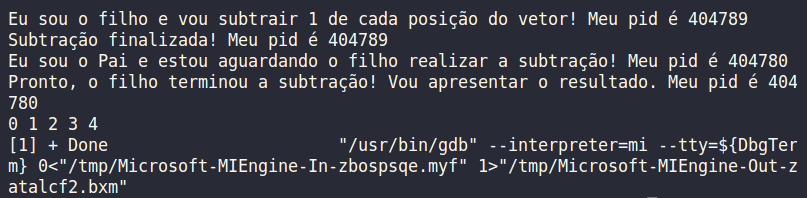
\includegraphics{q2_out}

\subsection*{Explicação}
O programa primeiro printa a seguinte frase : "Eu sou o Pai estou prestes a ter um filho!". Indicando que nesse momento, quem está rodando é o processo pai e o processo filho ainda não existe. Após isso é utilizado o comando fork, onde é criado um novo processo que é o processo filho.\\
    A partir daí, os dois processos, pai e filho, são concorrentes. O output do programa acontece de acordo com as condições explicitadas no código:\\
    Se o processo que está rodando atualmente é o filho, a seguinte frase é printada: "Eu sou o filho e vou subtrair 1 de cada posição do vetor!", a subtração é executada e é printado: Subtração finalizada!".\\
    Caso o processo que está rodando é o pai, temos esse output: "Eu sou o Pai e estou aguardando o filho realizar a subtração!", e então o processo pai espera pelo término do processo filho.\\
    Depois que o processo filho é finalizado, dentro do processo pai a frase "Pronto, o filho terminou a subtração! Vou apresentar o resultado." é printada. E então, o valor do vetor G é apresentado com os valores originais.\\
Note que o vetor G foi criado antes do fork, portanto ele tem o mesmo valor para os dois processos nesse momento.
No caso do processo filho, é feita a subtração. Então o valor de G muda para {-1, 0, 1, 2, 3}. Mas não é apresentado, de acordo com o proposto no enunciado.
Já no processo pai, o valor de G apresentado é o original. Pois não houve a subtração, visto que ela só é feita no processo filho.



	% ----------------------------------------------------------
	% Finaliza a parte no bookmark do PDF
	% para que se inicie o bookmark na raiz
	% e adiciona espaço de parte no Sumário
	% ----------------------------------------------------------
	\phantompart

%---------------------------------------------------------------------
% INDICE REMISSIVO
%---------------------------------------------------------------------
\phantompart
\printindex


\end{document}